\documentclass[12pt, oneside]{article}   	% use "amsart" instead of "article" for AMSLaTeX format
\usepackage[top=.5in, bottom=.5in, left = .5in, right=.5in, headheight=14.5pt, includeheadfoot]{geometry}
%\usepackage[margin = 1in]{geometry}                		% See geometry.pdf to learn the layout options. There are lots.
\geometry{letterpaper}                   		% ... or a4paper or a5paper or ... 
%\geometry{landscape}                		% Activate for rotated page geometry
%\usepackage[parfill]{parskip}    		% Activate to begin paragraphs with an empty line rather than an indent
\usepackage{graphicx}				% Use pdf, png, jpg, or eps§ with pdflatex; use eps in DVI mode
								% TeX will automatically convert eps --> pdf in pdflatex		
\usepackage{amssymb}
\usepackage{amsmath}
\usepackage[shortlabels]{enumitem}
\setlist{leftmargin=5.5mm}
\usepackage{float}
\usepackage{tikz-cd}
\usepackage{subcaption}
\usepackage{slashed}
\usepackage{mathrsfs}

% Packages from other template
\usepackage[final]{microtype}
\usepackage[USenglish]{babel}
\usepackage{hyperref}
\usepackage[T1]{fontenc}

%\usepackage{titlesec}
%\titlespacing{\section}{0pt}{12pt}{4pt}

\usepackage[compat=1.0.0]{tikz-feynman}

\usepackage{bm}
\usepackage{bbm}
\usepackage{bbold}

\usepackage{simpler-wick}
\usepackage[makeroom]{cancel}

\usepackage{tikz-3dplot}
\usepackage{amsthm}
\theoremstyle{definition}
\newtheorem{definition}{Definition}[section]
\newtheorem{theorem}{Theorem}[section]
\newtheorem{corollary}{Corollary}[theorem]
\newtheorem{lemma}[theorem]{Lemma}

\newcommand{\N}{\mathbb{N}}
\newcommand{\R}{\mathbb{R}}
\newcommand{\Z}{\mathbb{Z}}
\newcommand{\Q}{\mathbb{Q}}

\newcommand{\RI}{\mathrm{RI}}
\newcommand{\Tr}{\text{Tr}}
\newcommand{\TrC}{\text{Tr}_{\text{C}}}
\newcommand{\TrD}{\text{Tr}_{\text{D}}}

\usepackage{simpler-wick}
\usepackage[compat=1.0.0]{tikz-feynman}   %note you need to compile this in LuaLaTeX for diagrams to render correctly

\usepackage{parskip}
    \setlength{\parindent}{0in}
    %\setlength{\parindent}{.25in}

\usepackage{fancyhdr}
    \renewcommand{\headrulewidth}{.85pt}
    \renewcommand{\footrulewidth}{.6pt}
    \pagestyle{fancy}
    \renewcommand{\sectionmark}[1]{\markboth{#1}{}}
    \fancyhf{}
    \fancyhead[R]{Patrick Oare}
    \fancyhead[C]{\fontsize{14}{16.8}\textbf{Topology in Lattice Gauge Theory}}
    \fancyhead[L]{8.323 S2022}
    \fancyfoot[C]{\vspace*{.15in}\thepage}

% PSet Sections
\iffalse
\usepackage[explicit]{titlesec}
    \titleformat{\section}{\vspace*{0pt}\fontsize{16}{19.2}\selectfont}{}{0in}{\textbf{#1}{\hrule height .7pt width .75\textwidth}}
    \titlespacing{\section}{.35in}{.5in}{\parskip}
    \titleformat{\subsection}{\fontsize{14}{16.8}\selectfont}{}{.5in}{\textbf{\uline{#1}}}
    \titlespacing{\subsection}{0pt}{.5in}{\parskip}
\fi

% make arrow superscripts
\DeclareFontFamily{OMS}{oasy}{\skewchar\font48 }
\DeclareFontShape{OMS}{oasy}{m}{n}{%
         <-5.5> oasy5     <5.5-6.5> oasy6
      <6.5-7.5> oasy7     <7.5-8.5> oasy8
      <8.5-9.5> oasy9     <9.5->  oasy10
      }{}
\DeclareFontShape{OMS}{oasy}{b}{n}{%
       <-6> oabsy5
      <6-8> oabsy7
      <8->  oabsy10
      }{}
\DeclareSymbolFont{oasy}{OMS}{oasy}{m}{n}
\SetSymbolFont{oasy}{bold}{OMS}{oasy}{b}{n}

\DeclareMathSymbol{\smallleftarrow}     {\mathrel}{oasy}{"20}
\DeclareMathSymbol{\smallrightarrow}    {\mathrel}{oasy}{"21}
\DeclareMathSymbol{\smallleftrightarrow}{\mathrel}{oasy}{"24}
%\newcommand{\cev}[1]{\reflectbox{\ensuremath{\vec{\reflectbox{\ensuremath{#1}}}}}}
\newcommand{\vecc}[1]{\overset{\scriptscriptstyle\smallrightarrow}{#1}}
\newcommand{\cev}[1]{\overset{\scriptscriptstyle\smallleftarrow}{#1}}
\newcommand{\cevvec}[1]{\overset{\scriptscriptstyle\smallleftrightarrow}{#1}}

\newcommand{\dbar}{d\hspace*{-0.08em}\bar{}\hspace*{0.1em}}

% to use a box environment, use \begin{answer} and \end{answer}
\usepackage{tcolorbox}
\tcbuselibrary{theorems}
\newtcolorbox{answerbox}{sharp corners=all, colframe=black, colback=black!5!white, boxrule=1.5pt, halign=flush center, width = 1\textwidth, valign=center}
\newenvironment{answer}{\begin{center}\begin{answerbox}}{\end{answerbox}\end{center}}

\usepackage{pdfpages}

\begin{document}
%\maketitle

%\includepdf[page=-]{Recitation7_handwritten.pdf}

%\newpage
%\clearpage
%\setcounter{page}{1}

These notes will focus on reviewing and understanding the connection between topology (specifically algebraic topology) and lattice gauge theory. At the moment, I'm still learning the applications of algebraic topology to lattice gauge theory, so there may not end up being an overarching narrative to this document; however, I'll see if I can cobble anything interesting together. We'll draw on a lot of resources: some may be pretty mathematical, and I'll try to break it down accordingly so that it's understandable from a physics point of view. The main motivation for these notes is Michael DeMarco's thesis~\cite{demarco_thesis}, and I'll do a lot of recapping and trying to translate the language in the thesis into the language of high-energy lattice gauge theory. 

\section{Homology and Cohomology}

\textbf{Homology} is a mathematical method used to study a topological space $X$ via a sequence of algebraic structures with maps between them. The idea of homology is to associate a sequence of groups $\{H_n(X)\}_{n\in\mathbb N}$ to each topological space $X$, where each homology group $H_n(X)$ is a homotopy invariant of $X$. As notation, we'll often interchangeably write:
\begin{equation}
	H_*(X) := \bigoplus_{n\in\mathbb Z} H_n(X)
\end{equation}
in place of $\{H_n(X)\}_{n\in\mathbb Z}$ to emphasize the fact that the homology group is a \textbf{graded group}, i.e. it has is a direct sum of subgroups which are indexed by $n\in\mathbb Z$. 

The way that homology groups arise is by considering an algebraic sequence called a \textbf{chain complex}, which is a sequence of groups $\{C_n\}$ equipped with maps $d_n : C_n \rightarrow C_{n - 1}$ (we'll usually suppress the index on $d$) such that $d_{n - 1}\circ d_n = 0$ (i.e. $d^2 = 0$ if we suppress the index). This looks like:
\begin{equation}\begin{tikzcd}
		...\arrow[r, "d"] & C_{n + 1}\arrow[r, "d"] & C_n\arrow[r, "d"] & C_{n - 1}\arrow[r, "d"] & ...
\end{tikzcd}\end{equation}
The special thing about a chain complex is the fact that $d^2 = 0$. This $d$ map is often called a \textbf{boundary} operator, and we'll see why in the next section. That $d^2 = 0$ means that for each $c\in C_{n - 1}$, $d (dc) = 0\in C_{n + 1}$, which implies that $dc\in \mathrm{ker}(d_n)$, i.e. $\mathrm{im}(d_{n - 1})\subset \mathrm{ker}(d_n)$. Any term which looks like $dc$ is always killed by the differential, i.e. any term in the image of $d$ is in the kernel of the next $d$. The interesting thing we can do with this is look at the terms that are killed by $d$ which \textit{do not} look like $dc$, i.e. to consider the quotient group:
\begin{equation}
	H_n = \mathrm{ker}(d_n) / \mathrm{im}(d_{n - 1}). \label{eq:homology_group_dfn}
\end{equation}
Different groups and boundary operators will yield different types of homology. We'll see in the next section how one specific type (simplicial complexes) gives us some natural information about the number of ``holes'' in a topological space. 

The other concept we'll be studying is cohomology, which is essentially the dualized version of homology. Cohomology is very similar to homology, except it has additional structure that comes in the form of a graded product, called a \textbf{cup product}\footnote{For differential forms, there is a natural cohomology called the de Rham cohomology, which is given its ring structure via the wedge product $\wedge$.}. We'll denote cohomology groups by $H^n(X)$, and the graded cohomology ring by 
\begin{equation}
	H^*(X) = \bigoplus_{n\in\mathbb Z} H^n(X). 
\end{equation}
The essential difference in how cohomology is defined is that it arises from a \textbf{cochain complex}, which is like a chain complex, except the maps $d^n : C^n\rightarrow C^{n + 1}$ go up in grade:
\begin{equation}\begin{tikzcd}
		...\arrow[r, "d"] & C^{n - 1}\arrow[r, "d"] & C^n\arrow[r, "d"] & C^{n + 1}\arrow[r, "d"] & ...
\end{tikzcd}\end{equation}
There are a few names for the maps $d^n$: \textbf{coboundary} maps and \textbf{differential} maps are the most common terminology. The coboundary maps also must satisfy $d^2 = 0$ for $C^*$ to be a valid cochain complex, and then we can construct cohomology groups in the analogous way to Eq.~\eqref{eq:homology_group_dfn}. Let's focus on a specific example of (co)homology: the (co)chain complex that arises from considering simplices on a space. 

\subsection{Simplicial homology}

Let $n > 0$ be some integer. The \textbf{standard $n$-simplex} $\Delta^n$ is the convex hull of the standard basis $\{e_0, ..., e_n\}$ of $\mathbb R^{n + 1}$, i.e. we have:
\begin{equation}
	\Delta^n := \left\{\sum_{k = 0}^n t_k e_k : \sum_{k = 0}^n t_k = 1, t_k\geq 0\right\}
\end{equation}
The numbers $(t_0, ..., t_k)$ are called \textbf{barycentric coordinates}. Geometrically, an $n$-simplex is just an $n$-dimensional hyper-triangle. A 0-simplex is a point, a 1-simplex is a line, a 2-simplex is a triangle, a 3-simplex is a triangular prism, and so on. 

\tdplotsetmaincoords{70}{70}
\begin{figure}[!t]
\begin{subfigure}[t]{0.3\textwidth}
\centering
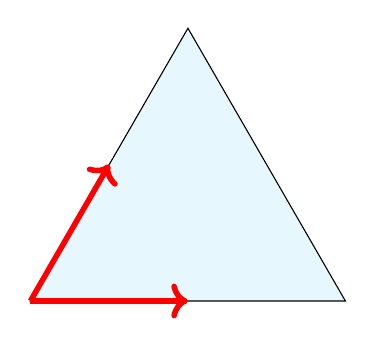
\begin{tikzpicture}
\draw[fill=cyan!10]
    (0,0)   -- coordinate (a) ++ 
    (+60:4) -- coordinate (b) ++ 
    (-60:4) -- coordinate (c) cycle;
\draw [->,red,line width=2pt]
    (0,0)  -- (a);
\draw [->,red,line width=2pt]
    (0,0)  -- (c);
%\draw[red] (a) -- (b) -- (c) -- cycle;
    \end{tikzpicture} 
    \caption{2-simplex.}
\end{subfigure}
\centering
\begin{subfigure}[t]{0.3\textwidth}
\centering
  \begin{tikzpicture}[scale=1,tdplot_main_coords,declare function={d=4;}]
     \path (0,0,0)       coordinate (A) 
         (d/2,d/2,0)     coordinate (H) 
          (d,0,0)        coordinate (C) 
            (d/2,{d*sqrt(3)/2},0)    coordinate (B) 
          (d/2,d/2,{d/sqrt(2)}) coordinate (D) 
          ($ (A)!0.5!(C) $) coordinate (M);
% \foreach \p in {A,B,C,H,D,M}
% \draw[fill=black] (\p) circle (1.5pt);
% \foreach \p/\g in {A/-90,B/-90,C/-90,D/90,H/-70,M/-135}
% \path (\p)+(\g:3mm) node{$\p$};
\draw (D) -- (A) (D) -- (B) (D) -- (C) (A) -- (C) -- (B);
\draw [dashed] (A) -- (B) (D) -- (H) (B) -- (M);
 \end{tikzpicture}
 \caption{3-simplex}
\end{subfigure}

\end{figure}

Let $X$ be any topological space. An \textbf{$n$-simplex} on $X$ is 

Simplicial homology is the study of how 

We'll begin with simplicial homology, which will be the main source of 

We begin with simplicial homology, which is a particular way to construct homology groups on a space. We 
will aim to study a space $X$ based on maps from simpler spaces (the $n$-simplices) into $X$.

\begin{definition}[Standard $n$-simplex]
	For $n > 0$, the \textbf{standard $n$-simplex} $\Delta^n$ is the convex hull of the standard basis 
	$\{e_0, ..., e_n\}$ of $\mathbb R^{n + 1}$, i.e. we have:
	\begin{equation}
		\Delta^n := \left\{\sum_{k = 0}^n t_k e_k : \sum_{k = 0}^n t_k = 1, t_k\geq 0\right\}
	\end{equation}
	The numbers $(t_0, ..., t_k)$ are called \textbf{barycentric coordinates}. 
\end{definition}

The standard $n$-simplex is an extraordinary simple space, and just looks like a hyper-triangle embedded 
into $\mathbb R^{n + 1}$. We can describe the $n$-simplex as an ordered pair $[v_0, ..., v_n]$, where 
each $v_i\in \{0, ..., n\}$ and none are repeated. This assigns each simplex an implicit orientation, and 
we can use this to manipulate such simplices. For each $n$, we have inclusion maps:
\begin{equation}
	d^i : \Delta^{n - 1}\rightarrow\Delta^n, \;\; 0\leq i\leq n
\end{equation}
where we map $[v_0, ..., v_{n - 1}]$ to $[v_0, ..., \hat v_i, ..., v_n]$, where the $\hat v_i$ denotes that we 
omit the vertex $v_i$. 

\begin{definition}[Singular $n$-simplex]
	Let $X$ be a topological space. Then a \textbf{singular $n$-simplex} is a map:
	\begin{equation}
		\sigma : \Delta^n\rightarrow X
	\end{equation}
	We define $Sin_n(X)$ to be the set of all singular $n$-simplices in $X$. 
\end{definition}

Note that the face maps induce a canonical map between the singular $n$-simplices on $X$ through the 
following composition of maps, which will call $d_i : Sin_n(X)\rightarrow Sin_{n - 1}(X)$, $\sigma\mapsto \sigma\circ d^i$:
\begin{equation}
	\begin{tikzcd}
		\Delta^{n - 1}\arrow[r, "d^i"]\arrow[dr, swap, "d_i\sigma"] & \Delta^n\arrow[d, "\sigma"] \\
		 & X
	\end{tikzcd}
\end{equation}
%$$
%	\Delta^{n - 1}\xrightarrow{d_i}\Delta^{n}\xrightarrow{\sigma} X
%$$

For $i\leq j$, the maps $d_i$ satisfy (and the face maps $d^i$ satisfy the same identity): 
\begin{equation}
	d_i d_j = d_{j + 1} d_i
\end{equation}

We wish to consider a variant of $Sin_n(X)$ which allows us to add and subtract simplices in a natural 
way. This will allow us to consider boundaries of simplices, which will be intimately connected to homology.  
For example, consider a 1-simplex which is a closed loop, i.e. $\gamma : [0, 1] = \Delta^1\rightarrow X$. 
We wish to be able to differentiate this loop from an open loop. We can almost do this with the definitions 
we have already made: notice that $d_0(\gamma) = \gamma(1) = \gamma(0) = d_1(\gamma)$. However, 
we need a way to take differences to make this precise. As such, we will consider the free abelian 
group generated by $Sin_n(X)$.
\begin{definition}[Singular $n$-chain]
	Let $S_n(X)$ be the free abelian group generated by $Sin_n(X)$:
	\begin{equation}
		S_n(X) := \mathbb Z Sin_n(X)
	\end{equation}
	We call an element of $S_n(X)$ a \textbf{singular $n$-chain}, and we may write each $n$-chain as:
	\begin{equation}
		\sum_{k = 1}^n a_k\sigma_k
	\end{equation}
	for $\sigma_k\in Sin_n(X)$. 
\end{definition}

\begin{definition}[Boundary operator]
	We define the \textbf{boundary operator} (also called a differential) $d : Sin_n(X)\rightarrow 
	S_{n - 1}(X)$ by:
	\begin{equation}
		\sigma\mapsto\sum_{i = 0}^n (-1)^i d_i\sigma
	\end{equation}
	This extends uniquely to a homomorphism:
	\begin{equation}
		d : S_n(X)\rightarrow S_{n - 1}(X)
	\end{equation}
\end{definition}

We will use this boundary map extensively, as it allows us to go between simplices of different dimensions. 
Intuitively, the boundary map just gives you the oriented face of the $n$-simplex; for example, the 
boundary of $\Delta^2$ is just an oriented (not filled in) triangle. Simplices which are killed by the 
differential are ``boundaries" of closed regions, in a sense which we will make precise.

\begin{definition}[$n$-cycle]
	An $n$-chain $c$ in $X$ is a \textbf{$n$-cycle} if $dc = 0$. We denote the set of all $n$-cycles by:
	\begin{equation}
		Z_n(X) := ker(d : S_n(X)\rightarrow S_{n - 1}(X)
	\end{equation}
\end{definition}

\begin{definition}[$n$-boundary]
	An $n$-chain $b$ in $X$ is a \textbf{$n$-boundary} if $b\in im(d)$. We denote the set of all 
	$n$-boundaries by:
	\begin{equation}
		B_n(X) := im(d : S_{n + 1}(X)\rightarrow S_n(X))
	\end{equation}
\end{definition}

\begin{theorem}
	The boundary operator satisfies:
	\begin{equation}
		d^2 = 0
	\end{equation}
	This implies that $B_n(X)\subseteq Z_n(X)$, so every boundary is a cycle. 
\end{theorem}

\begin{definition}[Graded abelian group]
	A \textbf{graded abelian group} is a sequence of abelian groups indexed by $\mathbb Z$. A 
	\textbf{chain complex} is a graded abelian group $\{A_n\}_{n\in\mathbb Z}$ together with 
	homomorphisms $d : A_n\rightarrow A_{n - 1}$ such that $d^2\equiv 0$. We will draw a chain 
	complex like so:
	\begin{equation}\begin{tikzcd}
			...\arrow[r, "d"] & A_{n + 1}\arrow[r, "d"] & A_n\arrow[r, "d"] & A_{n - 1}\arrow[r, "d"] & ...
	\end{tikzcd}\end{equation}
\end{definition}

An $n$-cycle in $Z_n(X)$ is closed in the way that a closed loop is closed-- it has no edges and all its 
faces connect with itself. The distinction between cycles and boundaries will give us homology groups. 
A nice way to visualize the difference is to consider an annulus in $\mathbb R^2$, $A = \{(x, y)\in\mathbb 
R^2 : x^2 + y^2\in [1, 3]\}$. A circle wrapping the annulus $x^2 + y^2 = 2$ is a cycle because it is a 
closed path; the boundary operator sends it to 0 since it links back to itself. However, it is \textbf{not} 
a boundary. It could almost be the boundary of $U := \{(x, y) : x^2 + y^2 \leq 2\}\cap A$, but this is not a 
simplex. $U$ is 2-dimensional and resembles the simplex $\Delta^2$, but unfortunately has a hole in it. 

In a manner such as this, homology will tell us about the holes that a space has by considering the 
quotient of the $n$-cycles by the $n$-boundaries. 

\begin{definition}
	For a topological space $X$, the $n$th \textbf{singular homology group} of $X$ is:
	\begin{equation}
		H_n(X) := Z_n(X) / B_n(X)
	\end{equation}
\end{definition}

Homology can also be defined in the same way for an arbitrary chain complex, and often once we have a 
chain complex we will forget about the underlying space it comes from. Note that homology groups 
$H_n(X)$ are always abelian, since $Z_n(X)$ is an abelian group. 

\begin{definition}[Semi-simplicial set]
	A collection of sets $K_n$ for $n\geq 0$ together with maps $d_i : K_n\rightarrow K_{n - 1}$ satisfying $d_i d_j = 
	d_{j + 1}d_i$ for $i\leq j$ is called a \textbf{semi-simplicial set}. 
\end{definition}

This notion generalizes the structure of the set $Sin_n(X)$. What we have done in the previous few pages is summarized 
as follows: to each topological space, we associate a semi-simplicial set $Sin_n(X)$. To each of these sets, we create the 
free abelian group $S_n(X)$ generated on these simplices. This forms a chain complex $(S_*(X), d)$, and we take the 
homology of said chain complex to form the homology of the space. 

For a basic computation, consider the homology of the one point space $X = \{*\}$. There is a single $n$ simplex for each 
$n$ because $X$ only has one point, which we will denote by $C_*^n$, so $S_*(X) = \mathbb Z\{C_*^n\}$. The composition 
of a face map with $C_*^n$ is $C_*^{n - 1}$ because we are simply sending the simplex of one dimension smaller to $*$, 
so $d_i C_*^n = C_*^{n - 1}$. But, this implies that:
\begin{equation}
	d C_*^n = \begin{cases}
		C_*^{n - 1} & n\textnormal{ even} \\
		0 & n\textnormal{ odd} \\
	\end{cases}
\end{equation}
because for odd $n$ we have an even number of face maps, so the alternating sum $d = \sum_{i = 0}^n (-1)^n d_i$ cancels 
itself and vanishes. For even $n$ we have one surviving $d_i$, so $d C_*^n = C_*^{n - 1}$. So, the chain complex of 
$n$-chains on $X$ is the following sequence (here I have labeled each copy of $\mathbb Z$ with which copy of $S_n(X)$ 
it is):
\begin{equation}\begin{tikzcd}
		...\arrow[r, "id"] & \mathbb Z\arrow[r, "0"] & \mathbb Z\arrow[r, "id"] & \mathbb Z\arrow[r, "0"]
		& \mathbb Z\arrow[r, "0"] & 0\arrow[r] & ... \\
		 & S_3(X) & S_2(X) & S_1(X) & S_0(X) &
\end{tikzcd}\end{equation}
For the even and nonzero $n$, the kernel of $id : S_n(X)\cong\mathbb Z\rightarrow \mathbb Z$ is 0, so $Z_n(X) = 0$ and 
hence $H_n(X) = 0$. Similarly for odd $n$, the kernel of $0 : \mathbb Z\rightarrow\mathbb Z$ is $\mathbb Z$, but the image 
of the previous map is $im(id) = \mathbb Z$, hence $Z_n(X) = B_n(X) = \mathbb Z$, so the homology $H_n(X)$ vanishes as 
well. However, for $n = 0$, we note that $Z_0(X) = \mathbb Z$ and $B_0(X) = \{0\}$, hence $H_0(X) = \mathbb Z$. 
Hence to summarize:
\begin{equation}
	H_n(*) = \begin{cases}
	0 & n > 0 \\
	\mathbb Z & n = 0
	\end{cases}
\end{equation}

We will now briefly consider the functorial nature of homology before 
moving on to lay out some definitions in category theory. 

\begin{definition}[Chain map]
	Let $C_*$ and $D_*$ be two chain complexes. A \textbf{chain map} $f_* : C_*\rightarrow D_*$ is a collection of 
	homomorphisms $f_n : C_n\rightarrow D_n$ such that the following diagram commutes:
	\begin{equation}\begin{tikzcd}
	...\arrow[r, "d"] & C_{n + 1}\arrow[d, "f_{n + 1}"]\arrow[r, "d"] & C_n\arrow[d, "f_n"]\arrow[r, "d"] & C_{n - 1}\arrow[d, 
	"f_{n - 1}"]\arrow[r, "d"] & ... \\
	...\arrow[r, "d"] & D_{n + 1}\arrow[r, "d"] & D_n\arrow[r, "d"] & D_{n - 1}\arrow[r, "d"] & ...
	\end{tikzcd}\end{equation}
\end{definition}

A chain map is just a sequence of maps which respect the differential. Now, we show that a continuous map from $X$ to $Y$ 
induces a chain map on the $n$-chains of $X$, which we will show in turn induces a morphism on homology. 

\begin{theorem}
	Let $f : X\rightarrow Y$ be a continuous map. Then $f$ induces a chain map:
	\begin{equation}
		f_* : S_*(X)\rightarrow S_*(Y)
	\end{equation}
\end{theorem}

\begin{proof}
	The induced map is very much a natural one, and we shall map the generators $\sigma$ of $S_n(X)$ to $\sigma\mapsto 
	f\circ\sigma : \Delta^n\rightarrow Y$, which extends to a homomorphism $f_* : S_*(X)\rightarrow S_*(Y)$ by linearity. We 
	must show that $f_*$ is in fact a chain map. We have:
	\begin{equation}
		d_i (f_*\sigma) = d_i (f\circ\sigma) = (f\circ\sigma)\circ d^i = f(d_i\sigma)
	\end{equation}
	hence summing this up, we see that $df_* = f_*d$. 
\end{proof}

\begin{theorem}
	Any chain map $f_* : C_*\rightarrow D_*$ induces a homomorphism on homology $f_* : H_*(C)\rightarrow H_*(D)$. 
\end{theorem}

\begin{proof}
	We will restrict each $f_n : C_n\rightarrow D_n$ to the $n$-cycles $Z_n(C)$ and show that the map $f_n : Z_n(C)
	\rightarrow Z_n(D)$ and is well defined. Suppose that $x\in Z_n(C)$, so $dx = 0$. Then $df_n(x) = f_{n - 1}(dx) = 0$ 
	because $f_*$ is a chain map, hence $f_n(x)\in ker (d : D_n\rightarrow D_{n - 1})$, and the map is well defined on the 
	n-cycles. Projecting $Z_n(D)$ onto the homology with the map $\pi_D : Z_n(D)\rightarrow H_n(D)$, we have the 
	diagram:
	\begin{equation}\begin{tikzcd}
		Z_n(C)\arrow[d, "\pi_C"]\arrow[r, "f_n"] & Z_n(D)\arrow[d, "\pi_D"] \\
		H_n(C)\arrow[r, dashed, "\tilde f_n"] & H_n(D)
	\end{tikzcd}\end{equation}
	and we will show that $\tilde f_n : H_n(C)\rightarrow H_n(D), [c]\mapsto \pi_D f_n(c)$, i.e. that we have a well defined 
	lift from the quotient. Suppose that $[c] = [c']\in H_n(C)$, so $c = c' + db$ for $b\in C_{n + 1}$. Then we must show that 
	$\tilde f([c]) = \tilde f([c']) + \tilde f([db]) = \tilde f([c'])$, so we have:
	\begin{equation}
		\tilde f([db]) = \pi_D f_n(db) = \pi_D (d f_{n + 1}b) = 0
	\end{equation}
	because $df_{n + 1} b\in B_n(D) = im(d : D_{n + 1}\rightarrow D_n)$. Hence the map is well defined, so we have a 
	valid morphism $H_n(C)\rightarrow H_n(D)$ for all $n$. 
\end{proof}

\section{Simplicial Homology and Cohomology}

\section{de Rham Cohomology}

\subsection{Connections between de Rham and simplicial cohomology}

\section{Cohomology in lattice gauge theory}

\newpage
\begin{thebibliography}{99}

\bibitem{demarco_thesis}
DeMarco, M. \textit{Chiral Phases on the Lattice}. cond-mat/2203.01427 (2022)

\end{thebibliography}

\end{document}